\chapter{Конструкторский раздел}
\section{Общая схема метода}
Задача распознавания эмоций по звучащей речи сводится к соотношению исходных данные на входе (аудиозаписи звучащей речи) к определенному классу на выходе (виду эмоции). На рисунке \ref{fig:idef1} представлена IDEF0-диаграмма первого уровня решаемой задачи.
\begin{figure}[H]
	\centering
	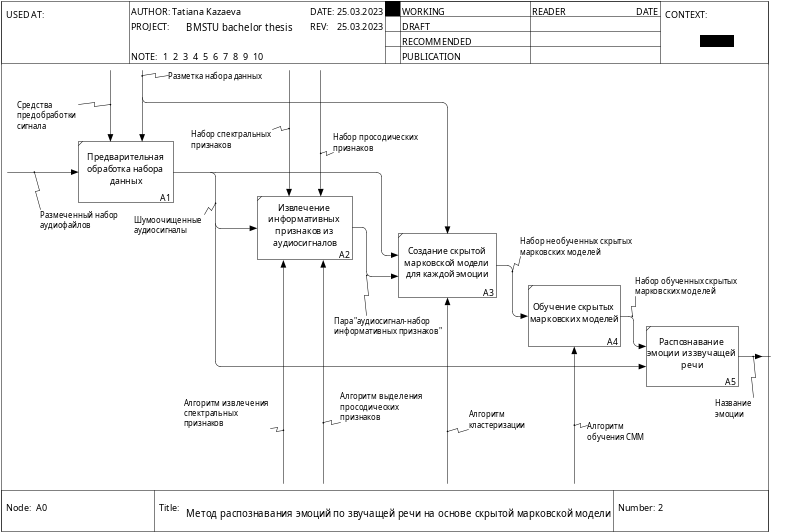
\includegraphics[width=\linewidth]{assets/02_A0.png}
	\caption{IDEF0-диаграмма первого уровня}
	\label{fig:idef1}
\end{figure}
Прежде всего набор данных должен быть предварительно обработан (блок А1).  Предварительная обработка включает в себя несколько этапов.
\begin{enumerate}
	\item Формирование соответствия <<аудиофайл-эмоция>> согласно разметке.
	\item Разделение набора данных на тренировочную (70-80\% набора) и тестовую (20-30\% набора) выборки. 
%	\item Для каждого аудиофайла: применение высокочастотных и низкочастотных пропускных фильтров, поскольку частота человеческого голоса лежит в диапазоне от 30 Гц до 2700 Гц. 
\end{enumerate}
Следующий этап решения задачи (блок А2) -- это выделение признаков из речевого сигнала. Поскольку сигнал должен быть разбит на кадры (фреймы) небольшой длительности, использование просодических признаков не имеет смысла, следовательно, будут использованы спектральные признаки речевого сигнала. 

Этап создания скрытой марковской модели для каждой эмоции (блок А3) включает в себя определение количества состояний модели, а также вероятностей перехода между состояниями и вероятностей наблюдения признаков в каждом состоянии. В качестве состояний модели используются типичные состояния речи (наборы численных значений выделенных спектральных и просодических признаков), которые определяются в результате кластеризации -- процесса группирования схожих признаков внутри набора данных.

Далее скрытая марковская модель обучается на тренировочной выборке данных (блок А4). Обученную марковскую модель можно использовать для распознавания эмоций в звучащей речи (блок А5).
%

\section{Описание используемого набора данных}
\subsection{Разметка и структура набора}
Для обучения классификатора было решено использовать набор данных DUSHA \cite{dusha}, содержащий записи эмоциональной речи. Набор разделен на два домена -- аудиоматериалы, собранные с помощью краудсорсинга (\textit{англ. <<Croud>>}) и выдержки из русскоязычных подкастов (\textit{англ. <<Podcast>>}). 

При разметке эмоциональных наборов данных существует сложность в неоднозначности интерпретации эмоции аннотаторами. В наборе данных DUSHA эта проблема решается привлечением к оцениванию двух независимых экспертных групп. В наборе присутствуют только те записи, для которых оценка обоих групп была консистентна. В разметке присутствуют следующие классы эмоций: 
\begin{itemize}
	\item \textbf{нейтраль};
	\item \textbf{позитив}: текст требовалось произносить с улыбкой или смехом, стараться делать выраженные ударения на позитивно окрашенных словах;
	\item \textbf{грусть}: произносить текст требовалось приглушенным голосом, меланхолично;
	\item \textbf{злость или раздражение}: текст требовалось произнести с криком или сквозь зубы, и, аналогично позитиву, стараться делать выраженные ударения на негативно окрашенных словах.
\end{itemize}

В домене <<Crowd>> тексты были искусственно сгенерированы на основе записей общения с голосовым ассистентом. Затем они были озвучены двумя способами: эмоционально, с той эмоцией, которую показал на этой записи классификатор BERT \cite{bert} и безэмоционально. Домен <<Podcast>> содержит уже не имитацию эмоции, а естественную речь. Все аудиозаписи были сделаны на профессиональные микрофоны, качество аудио было унифицировано до 16кГц. Аннототоры производили разметку, опираясь исключительно на звуковую дорожку, без учета произнесённого в ней текста.
\subsection{Содержание набора данных}
Поскольку разметку осуществляли несколько аннотаторов, требовалась агрегарция разметки. Она производилась по методу Дэвида --- Скина с порогом 0.9, выбранным эмпирически \cite{dusha}. Объём данных после агрегации с разбивкой по подмножествам приведён в таблице  \ref{tab:dusha-aggr}.
\begin{table}[H]
	\centering
	\caption{Объём данных после агрегации}\label{tab:dusha-aggr}
	\begin{tabular}{|c|P|P|P|P|}
		\hline
		\multirow{2}{*}{Домен} & \multicolumn{2}{c|}{Тренировочная выборка} & \multicolumn{2}{c|}{Тестовая выборка} \\ \cline{2-5} 
		& \multicolumn{1}{c|}{Файлы (шт.)} & Время & \multicolumn{1}{c|}{Файлы (шт.)} & Время \\ \hline
		Crowd & \multicolumn{1}{c|}{147057} & 184 ч. 21 мин. & \multicolumn{1}{c|}{13867} & 18 ч. 17 мин. \\ \hline
		Podcast & \multicolumn{1}{c|}{78810} & 70 ч. 08 мин. & \multicolumn{1}{c|}{10591} & 09 ч. 24 мин. \\ \hline
		Всего & \multicolumn{1}{c|}{225867} & 254 ч. 29 мин. & \multicolumn{1}{c|}{24458} & 27 ч. 41 мин. \\ \hline
	\end{tabular}
\end{table}
В агрегированном наборе данных имеются следующие поля разметки:
\begin{itemize}
	\item \textbf{audio\_path:} путь к аудиофайлу;
	\item \textbf{emotion:} эмоция, которую указал разметчик;
	\item \textbf{speaker\_text:} текст, который произнёс диктор (присутствует только в домене Crowd);
	\item \textbf{speaker\_emo}: эмоция, которую выражал диктор (присутствует только в домене Crowd);
	\item \textbf{source\_id}: уникальный идентификатор диктора или подкаста. 
\end{itemize}
\section{Проектирование отношений сущностей}
На каждом этапе  решения поставленной задачи формируется большой объем связанных структурированных данных, который необходимо хранить и дополнять. Для хранения этого набора решено использовать реляционную базу данных. На рисунке \ref{fig:chen} представлена диаграмма сущностей базы данных в нотации Чена.
\begin{figure}[H]
	\centering
	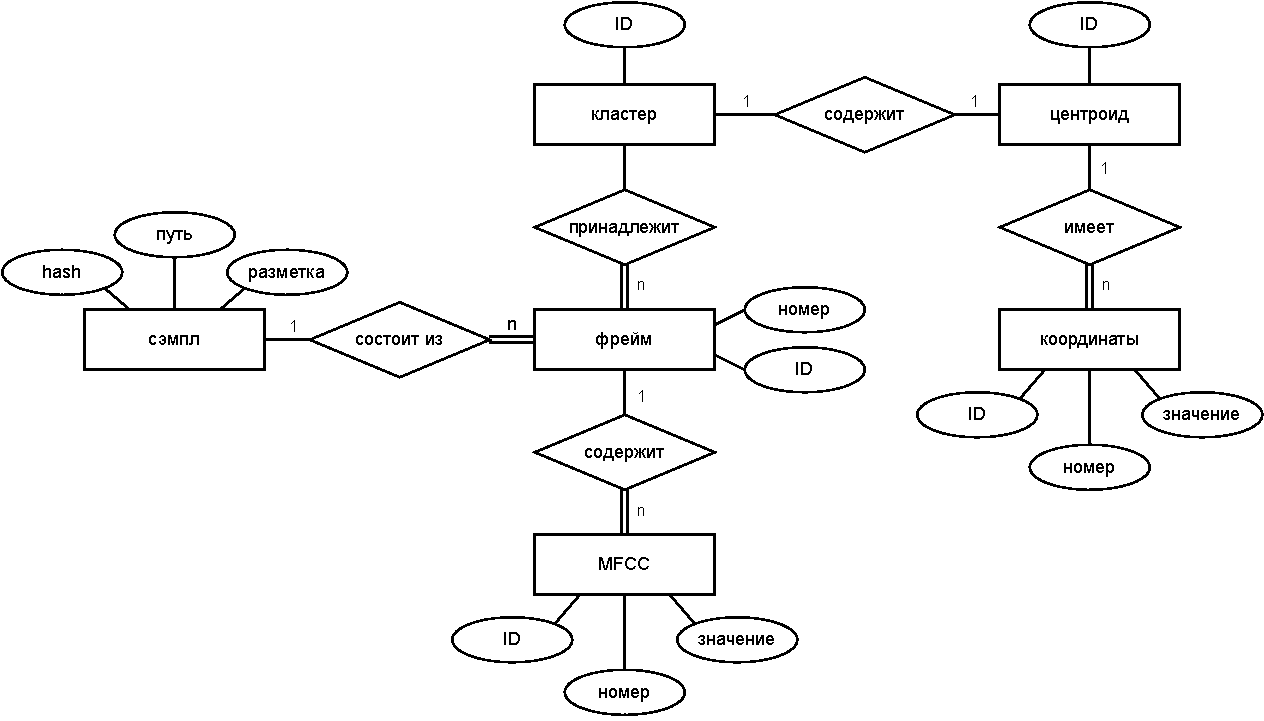
\includegraphics[width=\linewidth]{assets/chen}
	\caption{Диаграмма сущностей базы данных в нотации Чена}
	\label{fig:chen}
\end{figure} 
Сущность <<сэмпл>> представляет собой информацию о WAV-файле, который хранится в файловой системе. Сущность содержит поля, необходимые для ее обработки: уникальный хэш для идентификации сущности, абсолютный путь в файловой системе компьютера и разметка, указанная в корпусе. Звуковые дорожки разделены на небольшие фрагменты для дальнейшего анализа. Эти фрагменты представлены сущностью <<фрейм>>. Для работы с фреймами необходимо хранить информацию о его порядковом номере в сэмпле и идентификатор. 

Полученный набор фреймов используется в качестве входных данных для кластеризации. В результате кластеризации каждому фрейму присвоен кластер. Сущность базы данных, хранящая кластер, содержит уникальный идентификатор и информацию о своем центроиде. Центроид, в свою очередь, также содержит идентификатор и набор координат.

\section{Проектирование ключевых модулей системы}
%\subsection{Предварительная обработка данных}
%\subsection{Формирование обучающей выборки}
\subsection{Формирование вектора информативных признаков}
Самым надежным решением при распознавании эмоций в речи принято считать использование мел-кепстральных коэффициентов в качестве информативных признаков \cite{review}. В данной работе решено использовать первые 13 мел-кепстральных коэффициентов.

Входными данными модуля формирования вектора информативных признаков является набор сэмплов из корпуса DUSHA. Выходными данными являются фреймы каждого сэмпла и значения первых 13-ти мел-кепстральных коэффициентов на каждом фрейме.

Формирование вектора информативных признаков, состоящего из 13-ти первых мел-кепстральных коэффициентов представлено на рисунке \ref{fig:mfcc-vector}.
\begin{figure}[H]
	\centering
	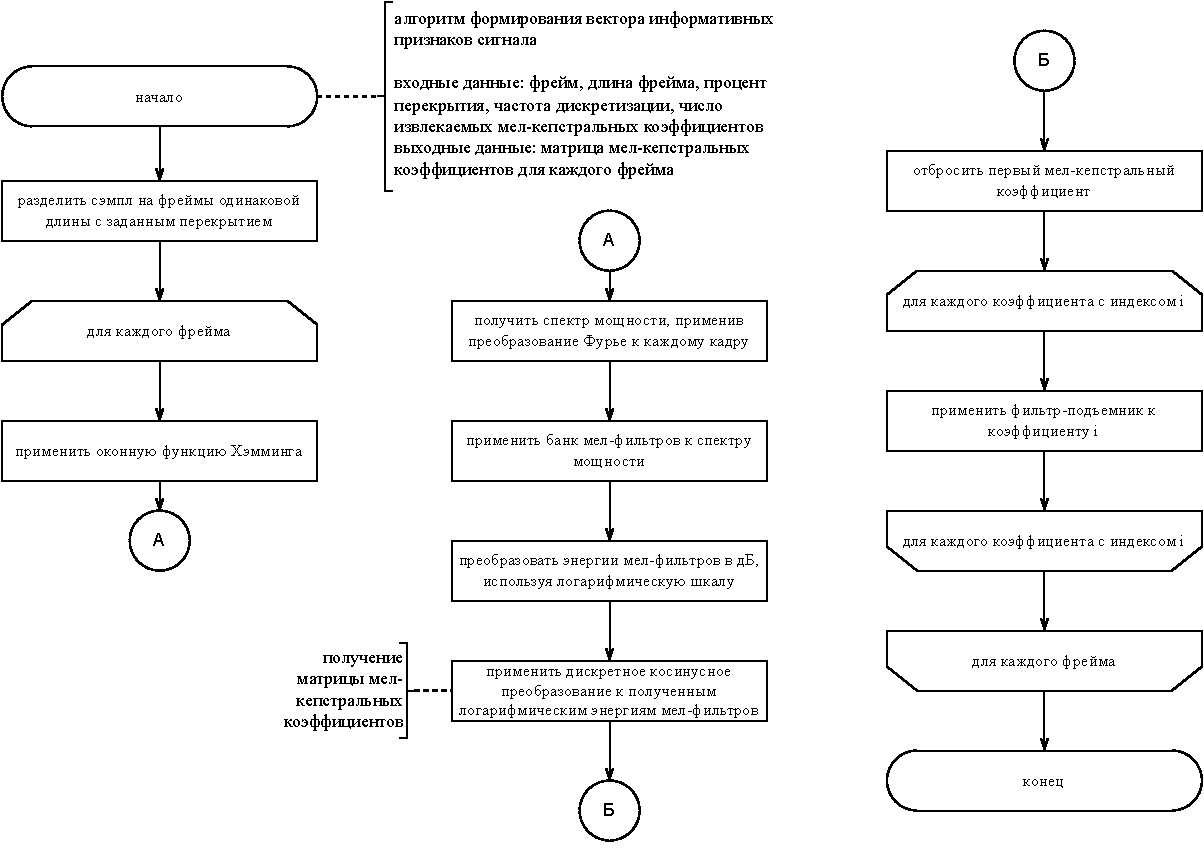
\includegraphics[width=\linewidth]{assets/mfccs-flowchart}
	\caption{Алгоритм формирования вектора информативных признаков}
	\label{fig:mfcc-vector}
\end{figure}

Фильтр-подъемник (lifter) применяется для усиления высокочастотных компонентов сигнала, которые могут быть утрачены в процессе преобразования сигнала в коэффициенты MFCC. Применение фильтра-подъемника происходит согласно \ref{eq:lifter}
\begin{equation}\label{eq:lifter}
	1 + \cfrac{\mathrm{lifter}}{2} \cdot \cfrac{\sin\left(\cfrac{\pi i}{\mathrm{lifter}}\right)}{1},
\end{equation}
где $i$ - индекс коэффициента MFCC, а $\mathrm{lifter}$ - значение параметра фильтра-подъемника.
\subsection{Кластеризация}
Для более эффективного процесса классификации с использованием скрытой марковской модели необходимо сократить размерность вектора входных данных. Для этого необходимо провести кластеризацию данных. В качестве алгоритма кластеризации был выбран k-means (\textit{англ. k-средних}).

Алгоритм k-means -- это неиерархичный метод неконтролируемого обучения. Он позволяет разделить произвольный набор данных на заданное число кластеров так, что объекты внутри одного кластера были достаточно
близки друг к другу, а объекты разных не пересекались. Цель этого алгоритма — объединить в группы сходные данные по некоторым заданным критериям. Чаще всего при кластеризации используются меры расстояния. В данной работе в качестве меры расстояния будет реализовано Евклидово (квадратичное) расстояние согласно \ref{eq:kdist}:
\begin{equation}\label{eq:kdist}
	\mathrm{dist}(p,\;q) = \sqrt{(p - q)^2},
\end{equation}
где $p, q$ -- точки вектора входных данных.

В качестве входных данных алгоритм принимает массив 13-ти мерных узлов, которые представляют собой значения мел-кепстральных коэффициентов, наблюдаемых на каждом фрейме каждого сэмпла. В качестве выходных данных -- массив 13-ти мерных узлов, являющихся центроидами каждого кластера, количество итераций для корректировки и количество кластеров, которое определяется эвристически. Схема алгоритма кластеризации представлена на рисунке \ref{fig:kmeans}.

\begin{figure}[H]
	\centering
	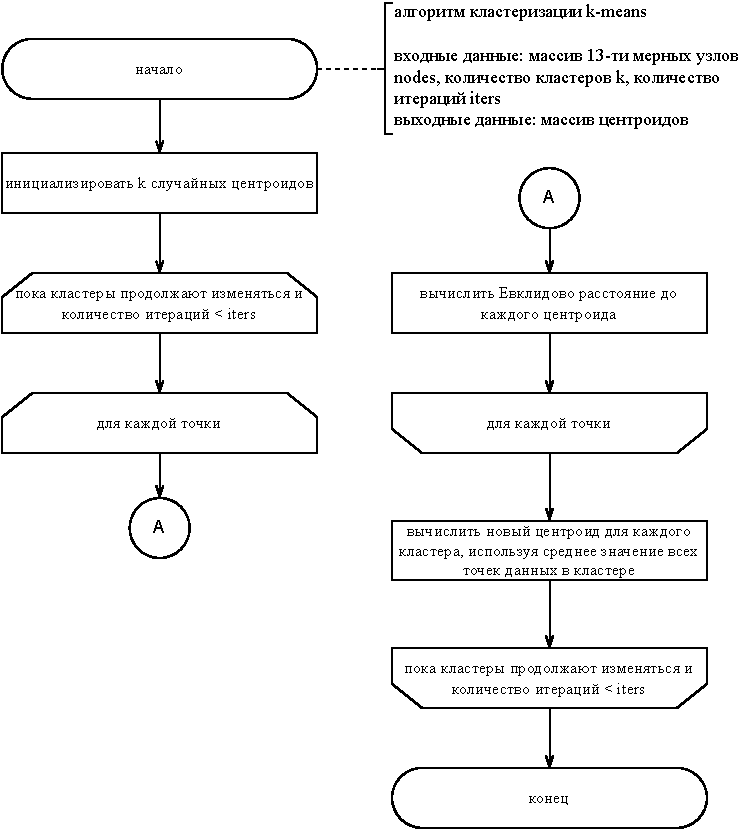
\includegraphics[width=0.75\linewidth]{assets/kmeans-flowchart}
	\caption{Алгоритм кластеризации k-means}
	\label{fig:kmeans}
\end{figure}

\subsection{Создание и обучение скрытых марковских моделей}
Обучение скртыой марковской модели -- это определение параметров $\lambda = \{A, B, \pi\}$ с учетом количества последовательностей наблюдений $\{O = O_1, \dots, O_n\}$. Для обучения скрытой  марковской модели используется алгоритм Баума --- Велша. Стоит отметить, что он применим только в том случае, если предварительно определено количество состояний и наблюдений.
%Алгоритм Баума-Велша состоит из трех этапов, для формализации которых следует ввести ряд обозначений.
Пусть $\gamma$ -- условная вероятность нахождения в определенном состоянии $q_i$ в с учетом последовательности наблюдений (\ref{hmm-gamma}):
\begin{equation}\label{hmm-gamma}
	\gamma_i = P(s_t = q_i\,|\,O,\,\lambda) = \cfrac{P(s_t = q_i,\,O\,|\,\lambda)}{P(O)}.
\end{equation}
Далее следует ввести переменную $\alpha$, обозначающую вероятность частичной последовательности наблюдений до момента времени $t$, находящаяся в состоянии $q_i$ в момент времени $t$, согласно \ref{hmm-alpha}:
\begin{equation}\label{hmm-alpha}
	\alpha_i = P(O_1, O_2, \dots, O_t,\, S_t = q_i\,|\,\lambda),
\end{equation}
и переменную $\beta$, вероятность частичной последовательности наблюдений от $t + 1$ до $T$, при нахождении в состоянии $q_i$ в момент времени $t$ (\ref{hmm-beta}): 
\begin{equation}\label{hmm-beta}
	\beta_i = P(O_{t+1}, O_{t+2}, \dots, O_T,\, S_t = q_i\,|\,\lambda),
\end{equation}
С учетом этих обозначений следует ввести переменную $\xi$, обозначающую вероятность перехода из состояния $i$ в момент времени $t$ в состояние $j$ в момент времени $t + 1$ с учетом последовательности наблюдений $O$ согласно \ref{hmm-xi}:
\begin{equation}\label{hmm-xi}
	\xi_t(i,\,j) = \frac{\alpha_t(i)a_{i,\,j}b_j(O_{t+1})\beta_{t+1}(j)}{P(O)}.
\end{equation}
С учетом переменных $\alpha$ и $\beta$ (\ref{hmm-alpha} и \ref{hmm-beta}) задать $\xi$ удобнее согласно \ref{hmm-xi-alpha-beta}:
\begin{equation}\label{hmm-xi-alpha-beta}
	\xi_t(i,\,j) = \alpha_t(i)a_{i,\,j}b_j(O_{t+1}\beta_{t+1}(j) \bigg/ \sum_{i}\sum_{j}\alpha_t(i)a_{i,\,j}b_j(O_{t+1}\beta_{t+1}(j)
\end{equation}
\noindent Условно алгоритм Баума---Велша можно разделить следующие этапы:
\begin{itemize}
	\item выполнение прямого прохода, в результате которого вычисляются вероятности наблюдаемых последовательностей до каждого момента времени и вероятности переходов из одного скрытого состояния в другое;
	\item выполнение обратного хода, в результате которого вычисляются апостериорные вероятности скрытых состояний в каждый момент времени;
	\item оценка априорных вероятностей -- количество случаев нахождения в состоянии $i$ в момент времени $t$;
	\item оценка вероятностей наблюдений -- количество случаев нахождения в состоянии $j$ при количестве наблюдений $k$ по отношению к количеству случаев нахождения в состоянии $i$.
\end{itemize}

Алгоритм Баума-Велша можно формализовать согласно \ref{alg:baum-welch}.

\begin{algorithm}[H]
	\SetAlgoLined
	
	\KwData{Скрытая марковская модель $\lambda$; Последовательность наблюдений $O$; количество состояний $N$;  количество итераций $\mathrm{iters}$}
	инициализация $\alpha$, $\beta$, $\gamma$, $\xi$;
	
	$i \leftarrow 0$;
	\For{ i < $\mathrm{iters}$}
	{
		вычислить $\alpha$ алгоритмом прямого хода\;
		
		вычислить $\beta$ алгоритмом обратного хода\;
		
		$\xi_{ij} (t) = \cfrac{\alpha_i(t) a_{i,\,j} b_{j,\,k\;v(t+1) }\beta_j(t+1)}{\displaystyle\sum_{i=1}^{N} \displaystyle\sum_{j=1}^{N} \alpha_i(t) a_{i,\,j} b_{j,\,k\;v(t+1) }\beta_j(t+1)}$\;
		
		$\gamma_i(t) = \sum_{j=1}^N \xi_{ij}(t)$\;
		
%		// Оценка априорных вероятностей -- количество случаев нахождения в состоянии $i$ в момент времени $t$. \\
		$\hat{\pi_i} = \gamma_1(i)$\;
		
%		// Оценка вероятностей переходов -- количество переходов из состояния $i$ в состояние $j$ по отношению к количеству случаев нахождения в состоянии $i$. \\
		$\hat{a_{i,\,j}} = \cfrac{\displaystyle\sum_{t=1}^{T-1} \xi_{ij} (t)}{\displaystyle\sum_{t=1}^{T-1} \displaystyle\sum_{j=1}^{M} \xi_{ij} (t)}$\;
		
%		// Оценка вероятностей наблюдений -- количество случаев нахождения в состоянии $j$ при количестве наблюдений $k$ по отношению к количеству случаев нахождения в состоянии $i$ \\
		$\hat{b_{j,\,k}} = \cfrac{\displaystyle\sum_{t=1}^T \gamma_j(t) 1(v(t)=k)}{\sum_{t=1}^T \gamma_j(t) }$\;
		
%		// Обновление параметров модели \\
		$A \leftarrow \hat{A};\;B \leftarrow \hat{B};\;\pi \leftarrow \hat{\pi}$\;
		
	} %% END For{ i < $\mathrm{iters}$}{
	\caption{Алгоритм Баума --- Велша}
	\label{alg:baum-welch}
\end{algorithm}

Выполнение прямого прохода осуществляется используя алгоритм прямого хода. алгоритм состоит из трех основных частей: инициализация, индукция и завершение. На этапе инициализации определяются переменные $\alpha$ для всех состояний в начальный момент времени. На этапе индукции вычисляются значения $\alpha_{t + 1}(i)$ по значениям $\alpha_t(i)$. На этапе завершения вычисляется значение $P(O\,|\,\lambda)$ путем суммирования всех значений $\alpha_T$.

\begin{algorithm}[H]
	\KwData{Скрытая марковская модель $\lambda$; Последовательность наблюдений $O$; количество состояний $N$;  Количество наблюдений $T$}
	$i \leftarrow 0;\;$\For{ i < $T$}
	{
		$\alpha_1(i) = \pi_ib_i(O_1)$; // инициализация
	}

	$t \leftarrow 1;\;$\For{ t < $T$}
	{
		$j \leftarrow 0;\;$\For{ j < $N$}
		{
			$\alpha_t(j) = \displaystyle\sum_i\alpha_{t - 1}(i)a_{i,\,j}b_j(O_t)$ // индукция
		}
	}
	$P(O) = \displaystyle\sum_i\alpha_T(i)$
	\caption{Алгоритм прямого хода}
	\label{alg:forward}
\end{algorithm}
Алгоритм, с помощью которого осуществляется обратный ход, работает аналогично, но в нем инициализация и индукция начинаются с конца последовательности.
\subsection{Определение эмоции из аудиосигнала}
Определение эмоции из аудиосигнала -- это получение вектора вероятностей принадлежности объекта-аудиосигнала к тому или иному эмоциональному классу. В контексте классификации с использованием скрытой марковской модели задача сводится к получению наиболее вероятного состояния в каждом интервале времени. Метод получения оптимальной последовательности состояний известен как алгоритм Витерби.

Для того, чтобы рассмотреть алгоритм Витерби, требуется ввести переменную $\delta$ согласно \ref{hmm-delta}:
\begin{equation}\label{hmm-delta}
	\delta_t(i) = \max\left[P(s_1, s_2, \dots, s_t = q_i, o_1, o_2, \dots, o_t\;|\;\lambda)\right],
\end{equation}
которая обозначает максимальное значение вероятности частичной последовательности состояний и наблюдений до момента времени $t$ при нахождении в состоянии $q_i$ в момент времени $t$. Как и в случае алгоритма прямого хода, задача решается итеративно. Итеративное нахождение значения $\delta$ происходит согласно \ref{hmm-delta-iter}:
\begin{equation}\label{hmm-delta-iter}
	\delta_{t + 1}(i) = \left[\max\left(\delta_t(i), a_{i,\,j}\right)\right]b_j(o_{t+1}).
\end{equation}

Алгоритм Витерби состоит из четырех этапов: инициализация, рекурсия, завершение и обратный проход. Для восстановления последовательности при обратном проходе после этапа завершения требуется ввести переменную $\psi_t$, в которой для каждого состояния $i$ в каждый момент времени t хранится предыдущее состояние, для которого была определена максимальная вероятность. 

Алгоритм Витерби может быть формализован согласно \ref{alg:viterbi}. 

\begin{algorithm}[H]
	\SetAlgoLined
	
	\KwData{Скрытая марковская модель $\lambda$; Последовательность наблюдений $O$; количество состояний $N$}
%	инициализация $\alpha$, $\beta$, $\gamma$, $\xi$;
	
	$i \leftarrow 0$;
	\For{ i < $N$}
	{
		// инициализация
		
		
		$\delta_1(i) = \pi_ib_i(O_1)$\;
		
		
		$\psi_1(i) = 0$\;
		
	}

	$t \leftarrow 1$; \For{ t < $T$}
	{
		$i \leftarrow 1$\;
		\For{ j < $N$}
		{
			// рекурсия
			
			
			$\delta_t(j) = \max\left[\delta_{t - 1}a_{i,\,j}\right]b_j(O_t)$\;
			
			
			$\psi_t(j) = \argmax_i\left[\psi_{t - 1}(i)a_{i,\,j}\right]$\;
			
		}
		
	}
	// завершение
	
	$P^{*} = \max_i\left[\delta_T(i)\right]$\;
	
	$q_T^* = \argmax\left[\psi_t(\delta_T(i))\right]$\;
	
	$i \leftarrow T$;
	\For{ j > 2}
	{
		// обратный проход
		
		
		$q_{t - 1}^* = \psi_t(q_{t}^*)$\;
		
	}
	 
	\caption{Алгоритм Витерби}
	\label{alg:viterbi}
	\end{algorithm}
%sum := 0.0
%for i := 0; i < len(hmm.A); i++ {
%	gamma[t][i] = alpha[t][i] * beta[t][i]
%	sum += gamma[t][i]
%}
%for i := 0; i < len(hmm.A); i++ {
%	gamma[t][i] /= sum
%}

%\begin{enumerate}
%	\item Оценка априорных вероятностей – количество случаев нахождения в состоянии $i$ в момент времени $t$ ():\\
%	\begin{equation}\label{hmm-pi}
%		\pi = 
%	\end{equation}
%	\item 
%	\item 
%\end{enumerate}

%Алгоритм состоит из двух этапов. На первом этапе выполняется прямой ход, в результате которого вычисляются вероятности наблюдаемых последовательностей до каждого момента времени и вероятности переходов из одного скрытого состояния в другое. На втором этапе выполняется обратный ход, в результате которого вычисляются апостериорные вероятности скрытых состояний в каждый момент времени.

%$P(q_t | O) = \cfrac{P(O_1, O_2, ..., O_t, q_t) \cdot P(O_{t+1}, O_{t+2}, ..., O_T | q_t)}{P(O_1, O_2, ..., O_T)}$

%вычисления апостериорных вероятностей скрытых состояний в скрытой марковской модели с известными параметрами модели
%\subsubsection{Кластеризация}
%В скрытой марковской модели для распознавания эмоций в речи скрытые состояния отображают различные эмоциональные состояния, а наблюдаемые состояния представляют собой информативные характеристики речи.
%
%Для определения количества состояний модели и вероятностей перехода между ними можно использовать методы, такие как анализ скользящего окна. Метод анализа скользящего окна включает в себя разбиение речевого сигнала на короткие временные интервалы (обычно около 10 мс) и вычисление информативных признаков речи для каждого интервала. Затем производится кластеризация признаков, чтобы определить наиболее типичные состояния речи, и их количество можно использовать в качестве количества состояний модели. Вероятности перехода между состояниями могут быть определены на основе статистических данных, полученных из тренировочной выборки.
%\subsection{Модуль обучения скрытых марковских моделей}
%\subsection{Модуль предварительной обработки набора данных}
%\subsection{Модуль выделения информативных признаков}
%%\subsection{Модуль создания и обучения классификатора}
%\section{Классификатор на основе скрытой марковской модели}
%\subsection{Создание скрытой марковской модели}
%\subsection{Обучение скрытой марковской модели}
%%\subsection{Обучение}
\section{Проектирование клиентского приложения}
\section{Вывод}